% !TEX root = ../report.tex
% Every number in this section comes from data/task1 via report/task1.py (which prints them), for the code
% defaults: IP table 16 sets x 6 ways, 9-bit signature, 512-entry pattern table, no prefetch distance.
% The data/task1/spp directory is NOT used: it ran an earlier SPP (64x4 IP table, 1024-entry pattern table).
\task{1}{Stride Pattern Prefetching}

\subsection{Task 1A: IP-stride prefetcher}
% TODO

\subsection{Task 1B: Design}

The prefetcher (\texttt{prefetcher/spp.l1d\_pref}) sits at the L1D and works on the cache-line strides of each load IP. It never prefetches outside the 4\,KB page of the access that triggers it. It has three tables:
\begin{enumerate}
  \item an \textbf{IP table} (16 sets $\times$ 6 ways, LRU) that holds each tracked IP's uniform stride and stride signature,
  \item a \textbf{pattern table} (512 entries, direct mapped) from a signature to the stride that followed it,
  \item a \textbf{recent-prefetch filter} (256 entries, direct mapped) that drops repeat requests and measures accuracy.
\end{enumerate}

\textbf{IP table.} An IP gets an entry on its first L1D miss. Once tracked, it trains on every load. Each entry keeps the low 16 bits of the IP's last line address, its last stride with a 2-bit confidence, a 9-bit stride signature, and a 2-bit chooser. A repeated line gives no new stride and is skipped. A stride larger than 63 lines always leaves the page, so it resets the entry's stride state.

\textbf{Two predictors per IP, chosen dynamically.} For each new stride $s$:
\begin{itemize}
  \item \emph{Uniform}: remember the last stride and predict that it repeats. Its confidence goes up when it repeats and down otherwise. The stored stride is replaced only at confidence 0, so one stray stride does not reset a stable one.
  \item \emph{Pattern}: predict the stride that followed the same recent stride history last time. Storing the last few strides of every IP raw, and a map from each history to its next stride, would be too large. Instead the history is hashed into a 9-bit signature, $\textit{sig} \leftarrow (\textit{sig} \ll 3) \oplus s$, with $s$ as 7-bit two's complement. Each new stride moves the older ones 3 bits up, so the signature covers the last 3 strides: the newest in 7 bits, the one before in 6, the one before that in 3. A pattern such as $(+1,+2,+2,+2,+3)^n$ needs exactly a history of 3 strides. After $(+2,+2)$ the next stride can be $+2$ or $+3$, but each of the five 3-stride histories has a single next stride.
  % TODO (data): no signature-length sweep is in data/. SIG_BITS / SIG_SHIFT are #defines, not env knobs, so a
  % sweep needs a knob or per-value builds. Show that 3 strides (9 bits) is enough on the traces, e.g. against 2 and 4.
\end{itemize}
A 2-bit chooser per IP starts at ``uniform'' and moves one step toward the predictor that was right whenever exactly one of them was. The uniform prediction is used when it is confident (confidence $\ge 2$) and the chooser is in its upper half, or when the pattern table has no confident prediction. Otherwise the pattern prediction is used. So uniform strides have priority, and an IP falls back to the pattern table only after the pattern table has been right where the uniform stride was wrong.

\textbf{Pattern table.} The 9-bit signature indexes the 512 entries directly. They are shared by all IPs. Each holds a 7-bit stride and a 2-bit confidence. The entries have no tag, so the same signature from two IPs shares an entry.
% TODO (design): add a tag to the pattern table.
% TODO (data): no PT_BITS sweep is in data/ (pending).
% TODO (code): pt_index() returns sig unmasked. It is correct only while SIG_BITS == PT_BITS; otherwise it indexes
% past the table. The static_assert there still says SIG_BITS <= 2 * PT_BITS ("folds the signature once"), which no
% longer guards it. Make it static_assert(SIG_BITS == PT_BITS), or restore the mask.

\textbf{Issuing.} The chosen predictor is walked ahead \emph{degree} steps: $L+s, L+2s, \dots$ for a uniform stride. For a pattern, each predicted stride is shifted into a copy of the signature to look up the next one. The walk stops at the first line outside the page, or at a pattern-table entry without confidence. A prefetch fills the L1D unless half of the L1D MSHRs are busy. In that case it fills only the L2.

\textbf{Recent-prefetch filter (RPF).} The RPF holds the lines requested recently, indexed by the low 8 bits of the line address with a 10-bit tag. A line already in it is not requested again. It also records whether each request has filled the L1D, which the accuracy checker uses (see Accuracy throttling).

\subsection{Storage overhead}

\begin{center}
\small
\begin{tabular}{@{}lrrr@{}}
\toprule
Structure & Entries & Bits per entry & Bits \\
\midrule
IP table & 96 & 52 & 4{,}992 \\
\multicolumn{4}{@{}l}{\quad valid 1, IP tag 12, last line (low bits) 16, stride 7,} \\
\multicolumn{4}{@{}l}{\quad stride confidence 2, signature 9, chooser 2, LRU 3} \\
Pattern table: stride 7, confidence 2 & 512 & 9 & 4{,}608 \\
Recent-prefetch filter: valid 1, line tag 10, filled 1 & 256 & 12 & 3{,}072 \\
Throttle: issued 9, useful 9, degree 4 & 1 & 22 & 22 \\
\midrule
Total & & & 12{,}694 bits $=$ 1{,}586.75 bytes \\
\bottomrule
\end{tabular}
\end{center}

Widths: a stride is at most $\pm 63$ lines, since a larger one always leaves the page, so it takes 7 bits. An IP is identified by 16 hashed bits: 4 pick the set and the other 12 are the tag. LRU among 6 ways needs 3 bits. The epoch counters count to 256, hence 9 bits. The degree goes up to 8, hence 4 bits.

\subsection{Accuracy throttling}

\textbf{Accuracy checker.} The RPF records whether each requested line has filled the L1D.
\begin{itemize}
  \item A prefetch is counted as issued once it fills the L1D.
  \item It is useful if a demand load reaches the line while the line is still in the RPF.
  \item A demand that misses on a requested line that has not filled yet is a late (or L2-only) prefetch. The prediction was right, so it counts as both issued and useful.
  \item A demand that hits on a requested line that never filled means the line was already cached. That prefetch was redundant and is not counted.
\end{itemize}
A prefetch that fills only the L2 is counted only if a demand reaches it, so an unused one is not seen.

\textbf{Degree control.} The degree is not fixed. It is chosen at run time. Every epoch of 256 counted prefetches, accuracy $a = \textit{useful}/\textit{issued}$ is compared with two thresholds. The degree goes up by one if $a \ge 0.75$, down by one if $a < 0.50$, and otherwise stays. It ranges from 1 to 8 and starts at 4. The degree the throttle settles on differs by trace:

\begin{center}
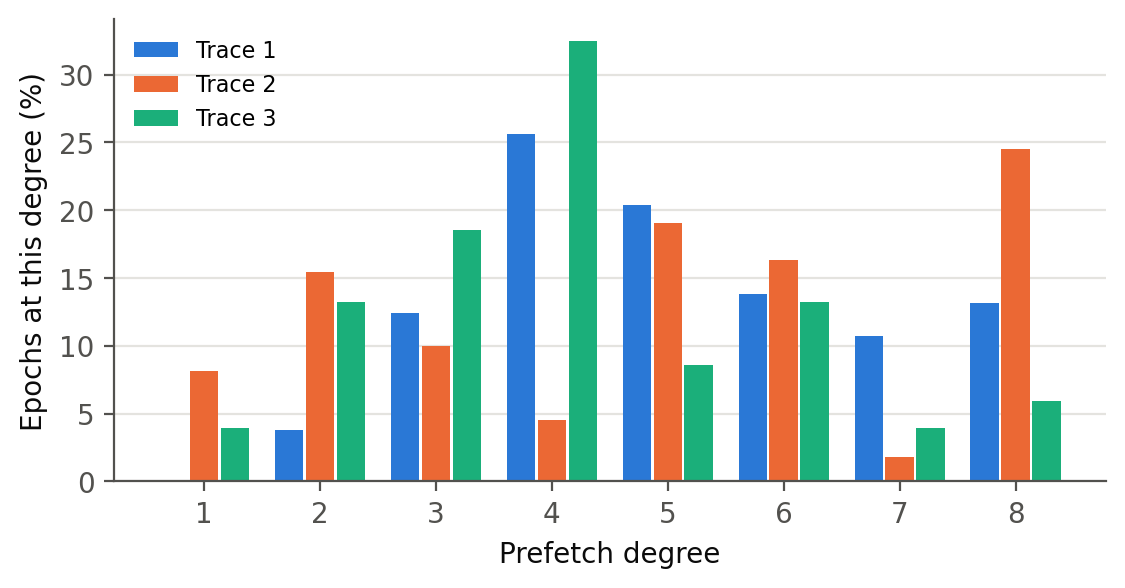
\includegraphics[width=0.6\textwidth]{t1_degree.png}
\end{center}

Trace2, where SPP is most accurate (65.2\%), spends the most epochs at the cap of 8 (24.5\%). Traces 1 and 3 spend most at degree 4 (25.6\% and 32.5\%).

\textbf{Why these thresholds.}
% TODO (deliverable, data): justify T_low = 0.50 and T_high = 0.75 from the mechanism (cost of a useless vs gain of a
% useful prefetch), and back it with a sweep on the current design. SPP_TLO and SPP_THI are env knobs, but no sweep of
% them on the current code is in data/.

\textbf{Why these degrees.}
% TODO (deliverable, data): justify the step of +-1, the floor of 1 (no prefetches means nothing to measure, so the
% degree could never come back up) and the cap of 8, with a sweep of the cap (SPP_DMAX is an env knob; no sweep of
% it on the current code is in data/). Use the histogram above: Trace2 sits at the cap for 24.5% of epochs.

\subsection{Results}

25M warmup and 25M simulated instructions per trace. The baseline has no L1D prefetcher and LRU at the L2C. Accuracy is ChampSim's: useful prefetches / prefetches issued to the L2. Mean: geometric for speedup, arithmetic otherwise.

\begin{center}
\begin{tabular}{@{}llrrrrr@{}}
\toprule
Trace & Prefetcher & IPC & Speedup & L1D load MPKI & Accuracy (\%) & Coverage (\%) \\
\midrule
Trace1 & none (baseline) & 0.2323 & 1.0000 & 10.68 & -- & -- \\
       & IP-stride       & 0.2335 & 1.0048 & 10.12 & 52.7 & 5.2 \\
       & SPP             & 0.2347 & 1.0102 &  9.45 & 55.8 & 11.5 \\
\midrule
Trace2 & none (baseline) & 0.2512 & 1.0000 & 13.54 & -- & -- \\
       & IP-stride       & 0.2513 & 1.0004 & 13.44 & 38.2 & 0.7 \\
       & SPP             & 0.2550 & 1.0153 & 12.88 & 65.2 & 4.8 \\
\midrule
Trace3 & none (baseline) & 0.3821 & 1.0000 &  3.40 & -- & -- \\
       & IP-stride       & 0.3829 & 1.0021 &  3.32 & 16.0 & 2.5 \\
       & SPP             & 0.3913 & 1.0242 &  2.74 & 49.4 & 19.6 \\
\midrule
Mean   & IP-stride       & 0.2892 & 1.0024 &  8.96 & 35.6 & 2.8 \\
       & SPP             & 0.2937 & 1.0165 &  8.36 & 56.8 & 12.0 \\
\bottomrule
\end{tabular}
\end{center}

\begin{center}
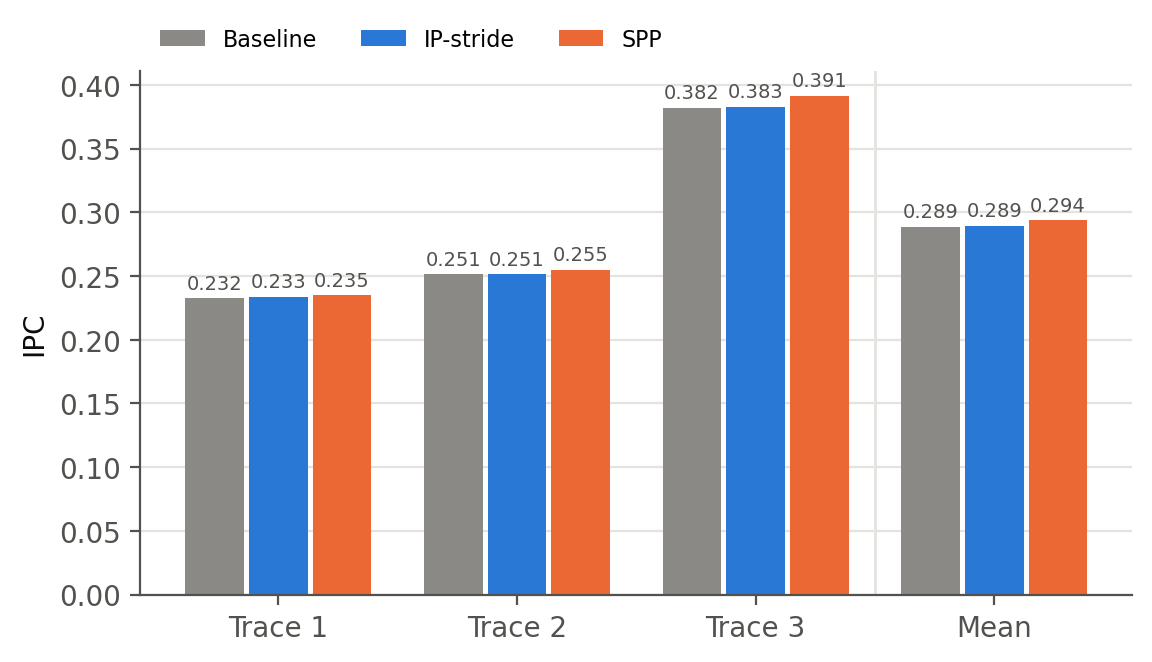
\includegraphics[width=0.32\textwidth]{t1_ipc.png}\hfill
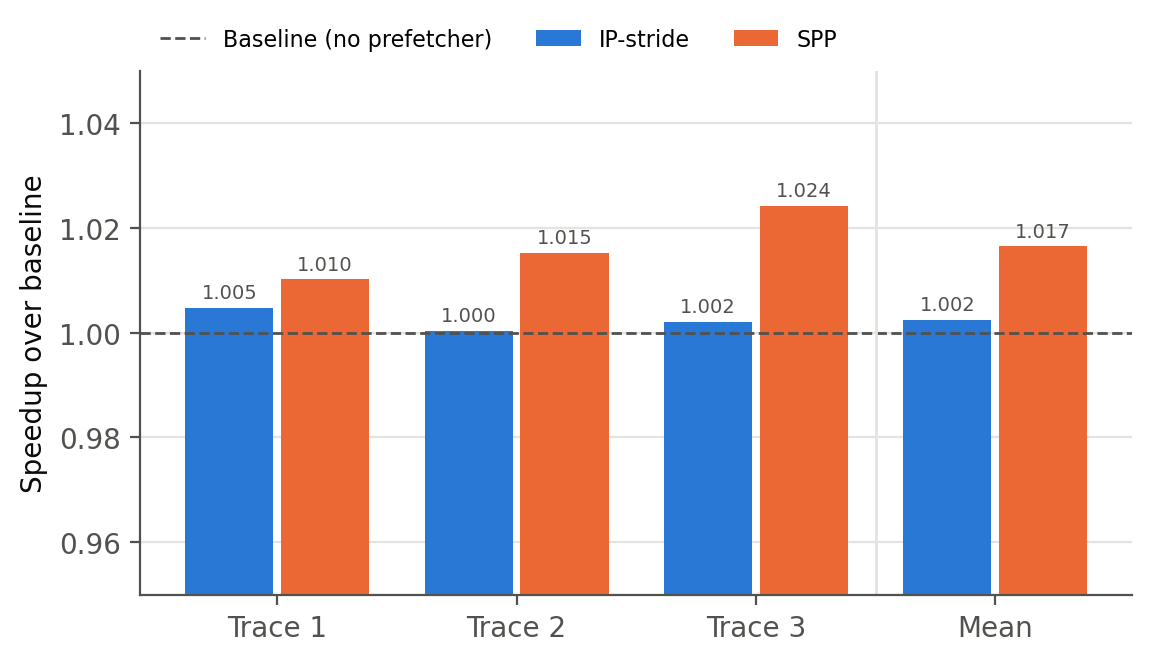
\includegraphics[width=0.32\textwidth]{t1_speedup.png}\hfill
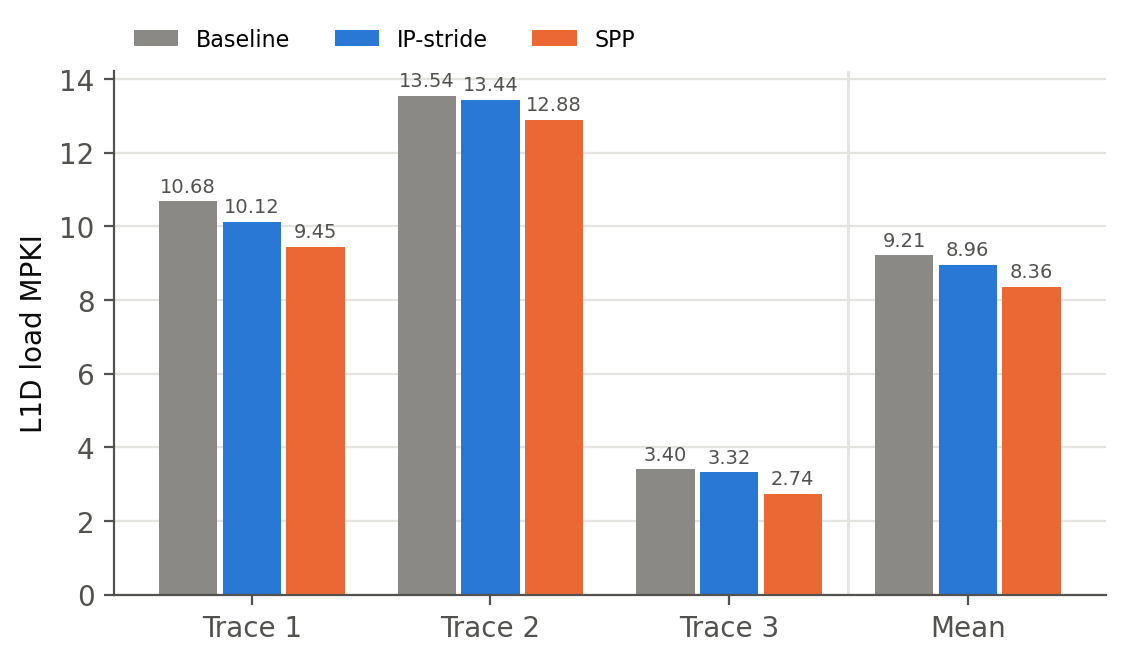
\includegraphics[width=0.32\textwidth]{t1_mpki.png}\\[0.4em]
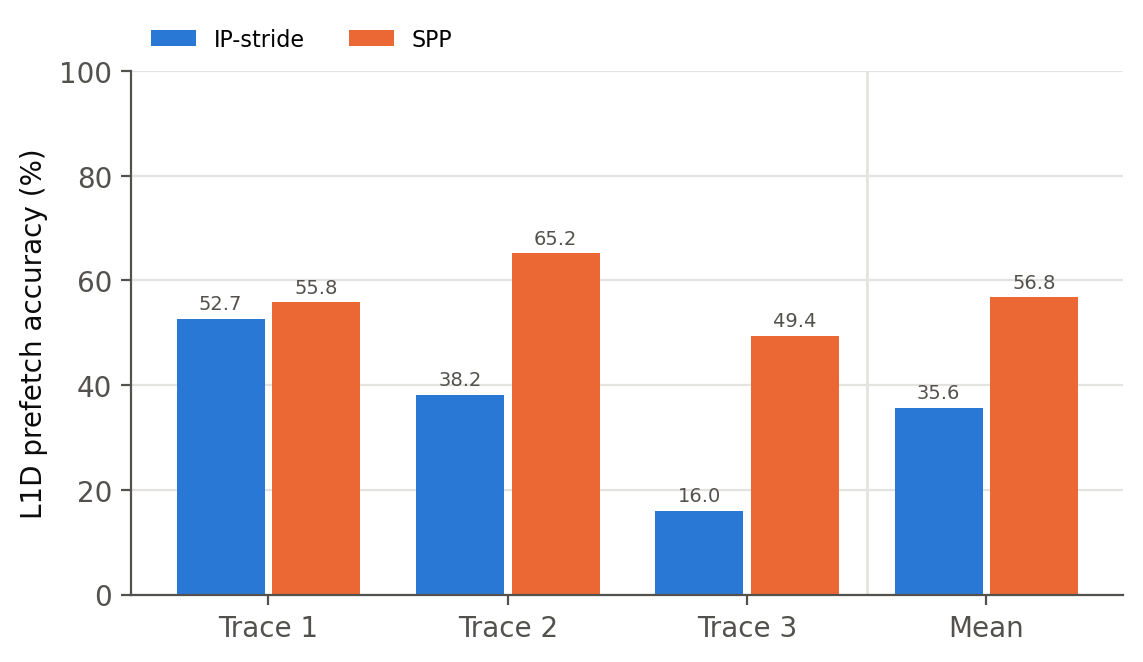
\includegraphics[width=0.32\textwidth]{t1_accuracy.png}\hfill
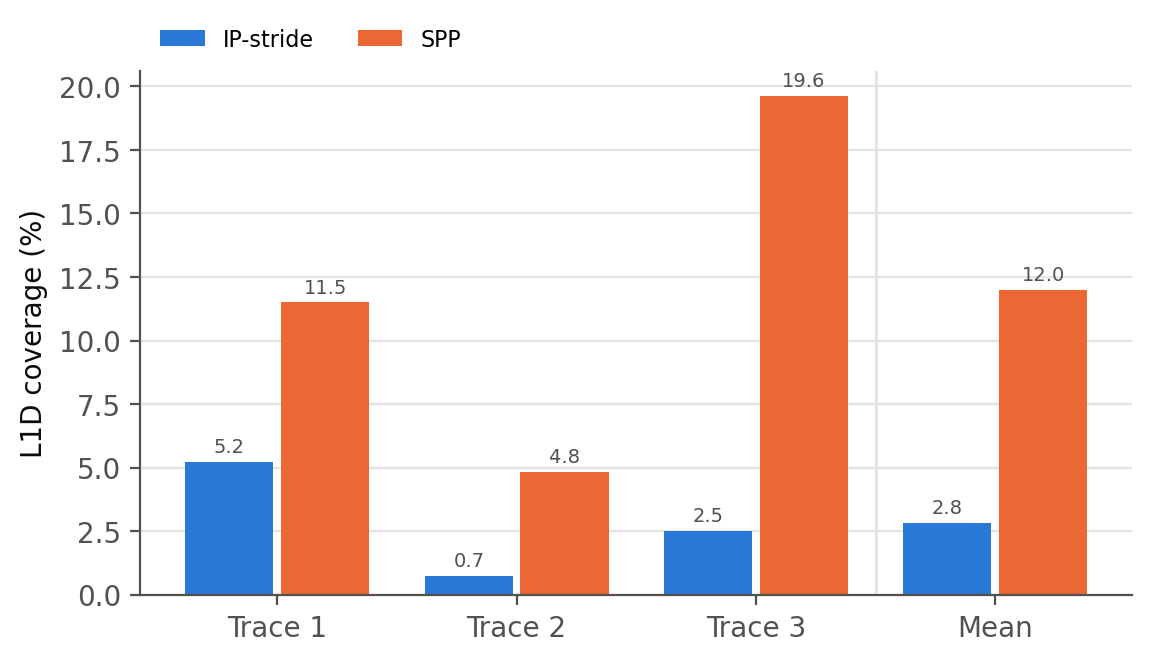
\includegraphics[width=0.32\textwidth]{t1_coverage.png}
\end{center}

SPP is faster than IP-stride on every trace, with higher accuracy and coverage on every trace.

\textbf{Uniform vs pattern.} Both predictors are used on every trace. The pattern table issues most of SPP's prefetches: 63\%, 79\% and 82\% on Traces 1--3. Its accuracy is lower than the uniform predictor's on Traces 1 and 2, and about the same on Trace3 (SPP's own accuracy checker):

\begin{center}
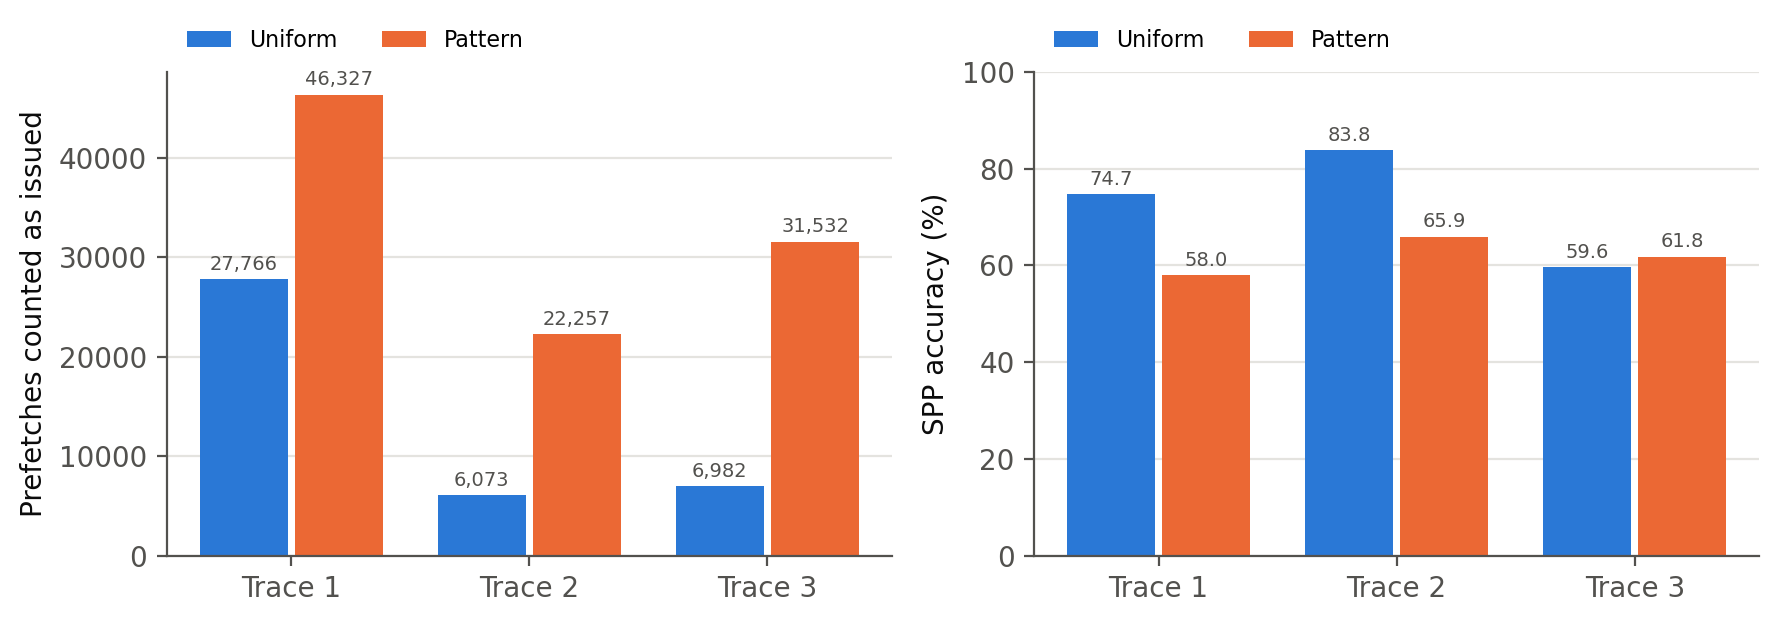
\includegraphics[width=0.75\textwidth]{t1_classes.png}
\end{center}

\textbf{Why the speedup is smaller than the coverage.} SPP removes 9\% of L1D load misses (mean MPKI 8.36 against 9.21) but gains 1.65\% IPC.
% TODO: explain. Data in the baseline logs: L1I MPKI 14.5, 40.0, 2.1 and branch MPKI 16.1, 6.3, 7.2 on Traces 1-3
% (frontend-bound?); Trace3, with the fewest L1I misses, gains most. Not yet a measured cause.

\subsection{Design choices}

\textbf{IP table size.} We swept the IP table's sets and ways, with SPP otherwise at its defaults:

\begin{center}
\begin{tabular}{@{}lrrrr@{}}
\toprule
Sets $\times$ ways & Entries & Speedup & Coverage (\%) & SPP storage (bytes) \\
\midrule
16 $\times$ 4 & 64 & 1.0160 & 11.97 & 1{,}370.75 \\
\textbf{16 $\times$ 6} & \textbf{96} & \textbf{1.0165} & \textbf{11.99} & \textbf{1{,}586.75} \\
32 $\times$ 4 & 128 & 1.0163 & 11.80 & 1{,}762.75 \\
16 $\times$ 8 & 128 & 1.0167 & 12.07 & 1{,}794.75 \\
32 $\times$ 6 & 192 & 1.0163 & 11.80 & 2{,}186.75 \\
64 $\times$ 4 & 256 & 1.0163 & 11.77 & 2{,}530.75 \\
32 $\times$ 8 & 256 & 1.0164 & 11.83 & 2{,}594.75 \\
64 $\times$ 6 & 384 & 1.0165 & 11.77 & 3{,}362.75 \\
64 $\times$ 8 & 512 & 1.0166 & 11.84 & 4{,}162.75 \\
\bottomrule
\end{tabular}
\end{center}

\begin{center}
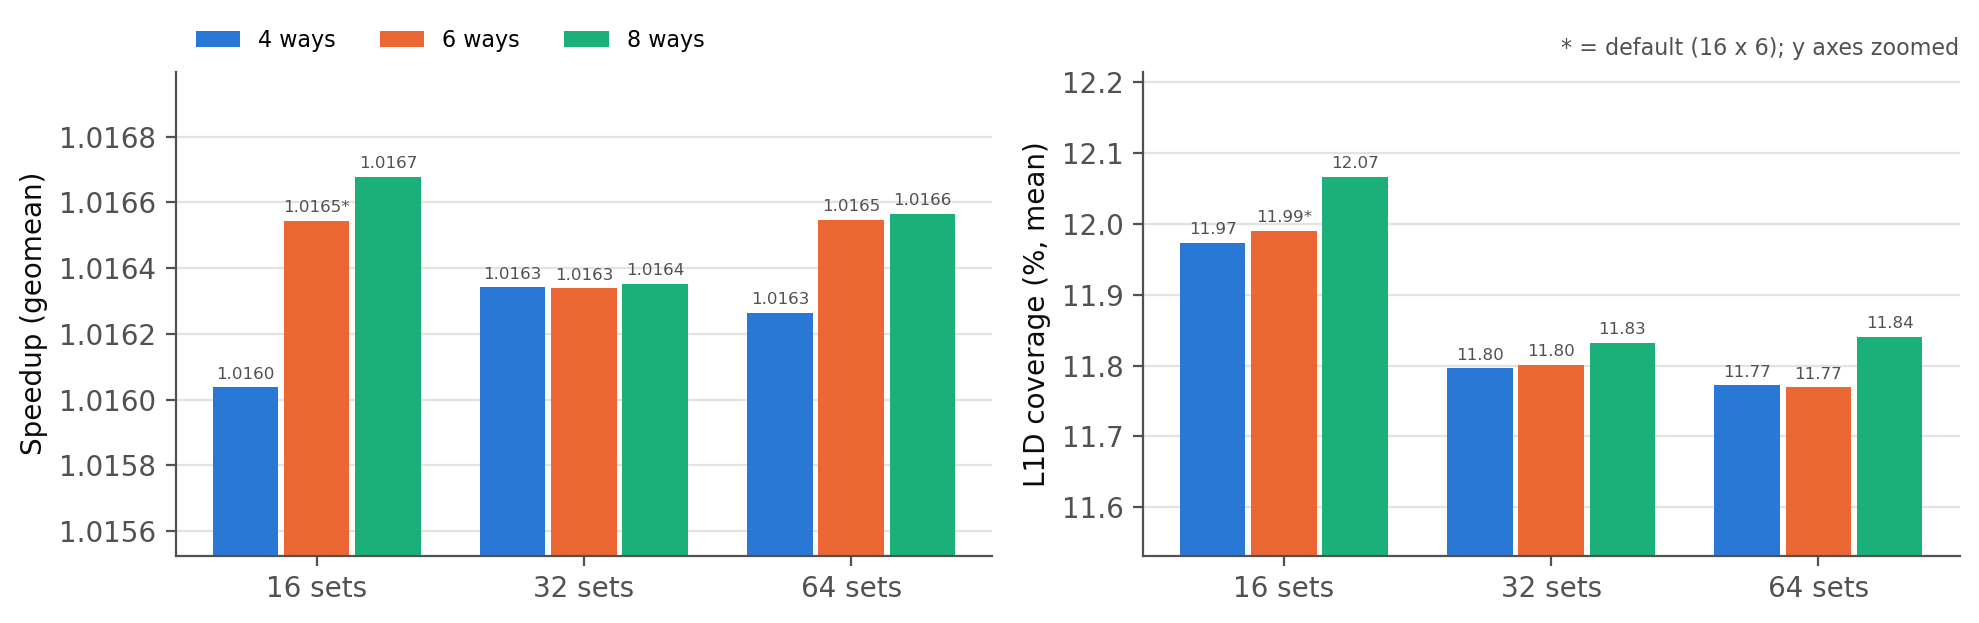
\includegraphics[width=\textwidth]{t1_ipt.png}\\[0.4em]
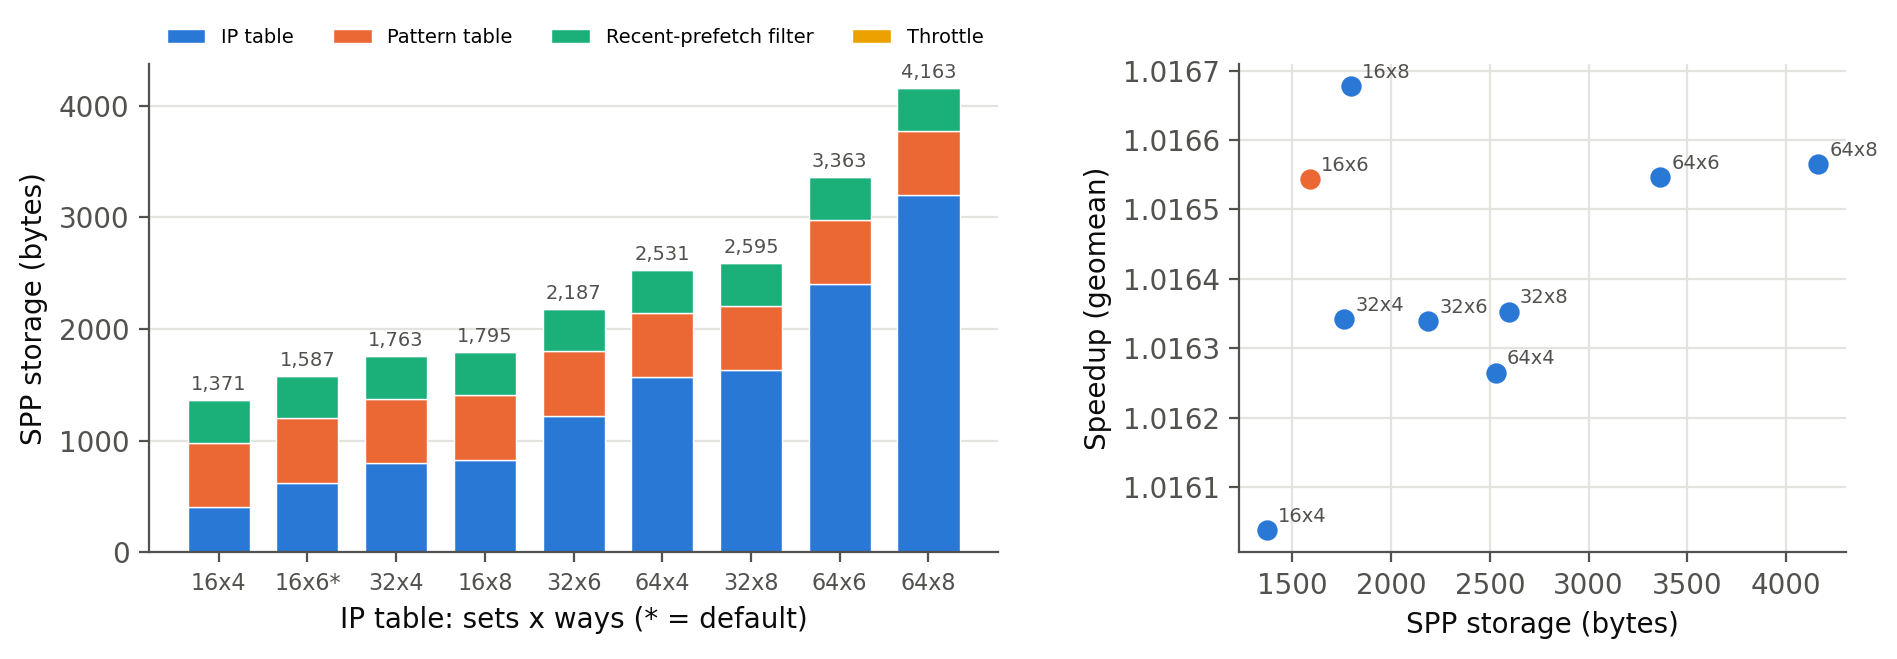
\includegraphics[width=\textwidth]{t1_storage.png}
\end{center}

All nine sizes are within 0.0007 of each other in speedup and 0.3 points in coverage, and a larger table does not help steadily. The IP table is the only structure whose size changes, from 30\% to 77\% of SPP's storage. We use 16 $\times$ 6: it is within 0.0002 of the best speedup, at 38\% of the storage of the largest table.
% TODO: the gaps between sizes are about as small as the change any edit causes (a different table changes which
% prefetches are sent, so the throttle's degree path differs). Say so, or test it.
% TODO: why size barely matters (allocation only on L1D misses keeps the table to IPs worth tracking?), and why the
% 16-set tables have slightly higher coverage. Not measured: count distinct allocated IPs.

\textbf{Prefetch distance (tried, not used).} To make prefetches less late, we tried a constant distance $d$: the walk goes $\textit{degree}+d$ steps ahead but issues only the last \emph{degree} of them, skipping the $d$ nearest lines. Lateness is the share of correct prefetches that arrive late (the L1D's late-prefetch counter over useful plus late). Means over the three traces, default IP table:

\begin{center}
\begin{tabular}{@{}rrrrr@{}}
\toprule
Distance $d$ & Speedup & Coverage (\%) & Accuracy (\%) & Late (\%) \\
\midrule
\textbf{0} & \textbf{1.0165} & \textbf{12.0} & \textbf{56.8} & \textbf{10.3} \\
1 & 1.0129 & 9.3 & 57.1 & 8.5 \\
2 & 1.0104 & 7.8 & 55.7 & 5.9 \\
3 & 1.0093 & 6.9 & 54.9 & 3.7 \\
4 & 1.0085 & 6.2 & 53.2 & 2.4 \\
\bottomrule
\end{tabular}
\end{center}

\begin{center}
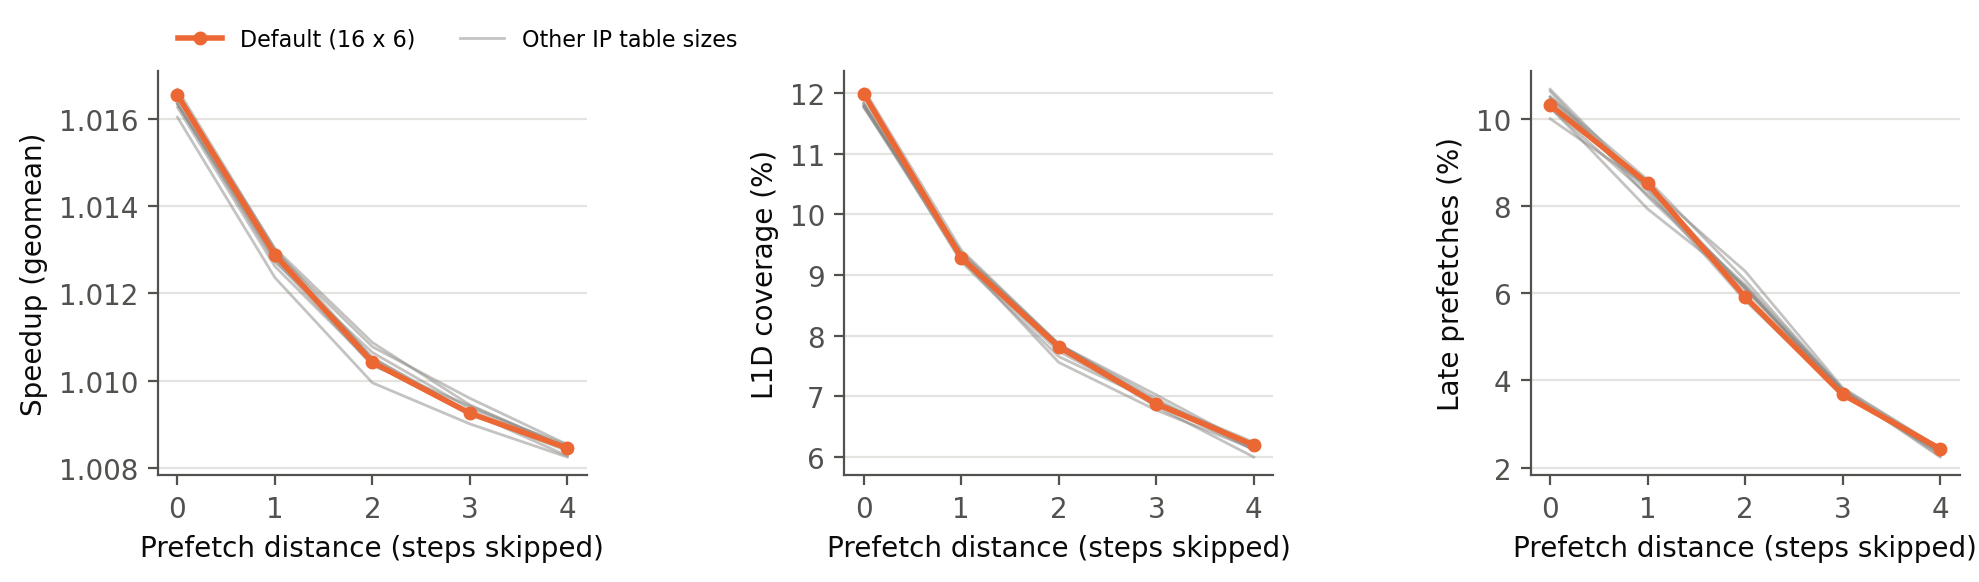
\includegraphics[width=\textwidth]{t1_distance.png}
\end{center}

A distance does cut lateness, but coverage halves (12.0\% to 6.2\% at $d = 4$), and speedup drops with every step, for all nine IP table sizes. Without a distance only 10.3\% of correct prefetches are late, so there was little to gain. We keep $d = 0$.
% TODO: why coverage falls (lines skipped at the start of each stream and lost at page ends?). Not measured.
% TODO (code, stats only): st_cand counts the skipped distance steps as candidates.
